  %
  % $Id:   $
  %
  % $Rev   ::                       $: Revision of last commit
  % $Author::                       $: Author of last commit
  % $Date  ::                       $: Date of last commit
  %
  % Author: Hans Skaug
  % Copyright (c) 2008 Regents of the University of California
  %
% Ting som m� sjekkes:
% - command line option for Linear model (se epost fra Dave).

% Not SW3.5
\documentclass[12pt,letter,reqno]{book}
\usepackage{amssymb}

%%%%%%%%%%%%%%%%%%%%%%%%%%%%%%%%%%%%%%%%%%%%%%%%%%%%%%%%%%%%%%%%%%%%%%%%%%%%%%%%%%%%%%%%%%%%%%%%%%%%
\usepackage{here,harvard,makeidx,hyperref}
\usepackage{graphicx,here}


%\textheight23cm
%\hoffset-1.3cm
%\voffset-1cm
%\textwidth16cm
%\parindent 0.7cm

\oddsidemargin=0.25in
\evensidemargin=0.25in
\textheight=8in
\textwidth=5.5in
%\hoffset=-0.0in
%\headheight=-0.0truein
%\headsep=0pt
%\topmargin=-.35truein
%\topskip=-2.75truein

\makeindex

\begin{document}

\title{ Random effects in AD Model Builder\\~ \\
	ADMB-RE user guide}
\author{admb-project.org}

\maketitle

\centerline{\LARGE License}
\input ../../../LICENSE

\newpage

\tableofcontents


\chapter{Introduction}

This document is a user's guide to random effects modelling in AD Model Builder (ADMB). Chapter~2 is a concise
introduction to ADMB, and Chapter~3 is a collection of examples selected from different fields of application.
Online program code and manuals are available from the ADMB Project at
admp-project.org, including
\begin{itemize}
\item The ADModel Builder manual
%\item \citeasnoun{skau:four:2004}, which describes the computational method used to handle random effect in 
\item Skaug and Fournier (2004), which describes the computational
method used to handle random effect in ADMB (http://bemata.imr.no/laplace.pdf).
\item The ADMB-RE example collection
\item The ADMB web-forum where you can ask questions to other users
(http: //www.otter-rsch.ca/phpbb/).
\end{itemize}
Why use AD Model Builder for creating nonlinear random effects models? The answer consists of three words --
flexibility, speed and accuracy. To illustrate these points a number of examples comparing ADMB-RE with two
existing packages NLME which runs on R and Splus, and WinBUGS. In general NLME is rather fast and it is good for
the problems for which it was designed, but it is quite inflexible. What is needed is a tool with at least the
computational power of NLME but the flexibility to deal with arbitrary nonlinear random effects models. In
section~\ref{lognormal} we consider a thread from the R user list where a discussion about extending a model to
use random effects which had a log-normal rather than normal distribution took place. This appeared to be quite
difficult. With ADMB-RE this change takes one line of code. WinBUGS on the other hand is very flexible and many
random effects models can be easily formulated in it. However, it can be very slow and it is necessary to adopt
a Bayesian perspective which may be a problem for some applications. 
A model which runs 25~times faster under ADMB than under WinBUGS may be found at:
\url{http://otter-rsch.com/admbre/examples/logistic/logistic.html}.


\section{Summary of features}

\paragraph{Model formulation}

With ADMB you can formulate and fit a large class of nonlinear statistical
models. With ADMB-RE you can include random effects in your model. Examples of such models include:
\begin{itemize}
\item Generalized linear mixed models (logistic and Poisson regression).
\item Nonlinear mixed models (growth curve models, pharmacokinetics).
\item State space models (nonlinear Kalman filter).
\item Frailty models in survival analysis.
\item Bayesian hierarchical models.
\item General nonlinear random effects models (fisheries catch-at-age
models).
\end{itemize}
You formulate the likelihood function in a template file, using a language that resembles C++. The file is
compiled into an executable program (Linux or Windows). The whole C++ language is to your disposal, giving you
great flexibility with respect to model formulation.

\paragraph{Computational basis of ADMB-RE}

\begin{itemize}
\item Hyper-parameters (variance components etc.)~estimated by maximum likelihood.
\item Marginal likelihood evaluated by the Laplace approximation or importance sampling.
\item Exact derivatives calculated using Automatic Differentiation.
\item Sampling from the Bayesian posterior using MCMC (Metropolis-Hastings algorithm).
\item Most features of ADMB (matrix arithmetic and standard errors, etc.) are available.
\end{itemize}

\paragraph{The strengths of ADMB-RE}

\begin{itemize}
\item \textit{Flexibility}: You can fit a large variety of models within a single framework.
\item \textit{Convenience}: Computational details are transparent. Your only
responsibility is to formulate the loglikelihood
\item \textit{Computational efficiency}: ADMB-RE is up to 50 times faster
than WinBUGS.
\item \textit{Robustness}: With exact derivatives you can fit highly nonlinear models.
\item \textit{Convergence diagnostic}: The gradient of the likelihood
function provides a clear convergence diagnostic.
\end{itemize}

\paragraph{Program interface}

\begin{itemize}
\item\textit{Model formulation}: You fill in a C++ based template
using your favorite text editor.

\item \textit{Compilation}: You turn your model into an executable program using
a  C++ compiler (which you need to install separately).

\item\textit{Platforms}: Windows and Linux
\end{itemize}

\paragraph{How to order ADMB-RE}

ADMB-RE is a module for ADMB. Both can be obtained from
admb-project.org

\chapter{The language and the program}

\section{What is ordinary ADMB?}

ADMB is a software package for doing parameter estimation in nonlinear
models. It combines a flexible mathematical modelling language (built on
C++) with a powerful function minimizer (based on Automatic
Differentiation). The following features of ADMB make it very useful for
building and fitting nonlinear models to data:

\begin{itemize}
\item Vector-matrix arithmetic, vectorized operations for common mathematical functions.
\item Read and write vector and matrix objects to file.
\item Fit the model is a stepwise manner (with `phases'), where more and more parameters become active in the minimization.
\item Calculate standard deviations of arbitrary functions of the model parameters by the `delta method'.
\item MCMC sampling around the posterior mode.
\end{itemize}
To use random effects in ADMB it is recommended that you have some experience in writing ordinary ADMB programs.
In this sections we review, for the benefit of the reader without this experience, the basic constructs of ADMB.

Model fitting with ADMB has three stages: 1) Model formulation, 2) Compilation and 3) Program execution.
The model fitting process is typically iterative: After having looked at the output from stage 3) one goes back to
stage 1) and modifies some aspect of the program.

\paragraph{Writing an ADMB program}
\index{tpl-file!writing}To fit a statistical model to data we must carry out certain fundamental tasks, such as
reading data from file, declaring the set of parameters that should be estimated, and finally we must give a
mathematical description of the model. In ADMB you do all of this by filling in a template, which is an ordinary
text file with the file-name extension `.tpl' (and hence the template file is known as the tpl-file). You
therefore need a text editor, such as 'vi' under Linux or 'Notepad' under Windows, to write the tpl-file. The
first tpl-file to which the reader of the ordinary ADMB manual is exposed is \texttt{simple.tpl} (listed
in~Section~\ref{sec:code example} below). We shall use \texttt{simple.tpl} as our generic tpl-file, and we shall
see that introduction of random effects only requires small changes to the program.

A tpl-file is divided into a number of `sections', each representing one of the fundamental tasks mentioned
above. The required sections are:
\begin{center}
\begin{tabular}{ll}
\textbf{Name} & \textbf{Purpose} \\ \hline
\texttt{DATA\_SECTION} & Declare `global' data objects; initialization from file \\
\texttt{PARAMETER\_SECTION} & Declare independent parameters \\
\texttt{PROCEDURE\_SECTION} & Specify model and objective function in C++
\end{tabular}
\end{center}
More details are given when we later look at \texttt{simple.tpl}, and a quick reference
card is available in Appendix~\ref{sec:quick}.

\paragraph{Compiling an ADMB program}

\index{tpl-file!compiling}After having finished writing \texttt{simple.tpl},
we want to convert it into an executable program. This is done in a
DOS-window under Windows, and in an ordinary terminal window under Linux. To
compile \texttt{simple.tpl}, we would under both platforms give the command:
\begin{verbatim}
    $ admb -re simple
\end{verbatim}
Here, '\texttt{\$}' is the command line prompt (which may be a different symbol on your computer), and
\texttt{-re} is an option telling the program \texttt{admb} that your model contains random effects. The program
\texttt{admb} accepts another option \texttt{-s} which produces the `safe' (but slower) version of the
executable program. The \texttt{-s} option should be used in a debugging phase, but it should be skipped when
the final production version of the program is generated.

The compilation process really consists of two steps: first \texttt{simple.tpl} is converted to a C++ program by
a preprosessor called \texttt{tpl2rem} (Appendix~\ref{sec:quick}). An error message from \texttt{tpl2rem} consists of a 
single line of text, with a reference to the line in the tpl-file where the error occurs. 
If successful, the first compilation step results in
the C++ file \texttt{\ simple.cpp}. In the second step \texttt{simple.cpp} is compiled and linked using an
ordinary C++ compiler (which is not part of ADMB). Error messages during this phase typically consist of long
printouts, with references to line numbers in \texttt{simple.cpp}. To track down syntax errors it may
occasionally be useful to look at the content of \texttt{simple.cpp}. When you understand what is wrong in
\texttt{simple.cpp} you should go back and correct \texttt{simple.tpl} and re-enter the command \texttt{admb -re
simple}. When all errors have been removed, the result will be an executable file, which is called
\texttt{simple.exe} under Windows or \texttt{simple} under Linux.

In some situations you may want to modify the options that are passed to the C++~compiler. The script~files
that actually invoke the compiler reside in the \texttt{bin} directory of your ADMB installation.
There are different versions of the scripts corresponding to the different combinations of command line options
you can invoke \texttt{admb} with. So, given that you type \texttt{admb~-re~-s} the compilation script~\texttt{myccsre}
will be called, and subsequently the linker script \texttt{mylinksre}. By looking
at the \texttt{bin} directory, or the contents of the script~\texttt{admb} which also resides
in this directory, you will easily figure out what is going on.
(Note that older version of ADMB used slightly different naming conventions.)

\paragraph{Running an ADMB-program}
\index{tpl-file!compiling}The executable program is run in the same window as it was compiled. Note that data
are not usually part of the ADMB program (\texttt{simple.tpl}). Instead, data are being read from a file with
the file name extension `.dat' (\texttt{simple.dat}). This brings us to the naming convention used by ADMB programs for
input and output files: The executable automatically infers file names by adding an extension to its own
name. The most important files are:
\begin{center}
\begin{tabular}{lll}
& \textbf{File name} & \textbf{Contents} \\ \hline
Input & \texttt{simple.dat} & Data for the analysis \\
& \texttt{simple.pin} & Initial parameter values \\ \hline
Output & \texttt{simple.par} & Parameter estimates \\
& \texttt{simple.std} & Standard deviations \\
& \texttt{simple.cor} & Parameter correlations
\end{tabular}
\end{center}
You can use command line options to modify the behavior of the program at runtime. The available command line options can be
listed by typing:
\begin{verbatim}
    $ simple -?
\end{verbatim}
(or whatever your executable is called). The command line options that
are specific to ADMB-RE are listed in Appendix 1, and are discussed in detail under the various sections. An
option you probably will like to use during an experimentation phase is \texttt{-est}, which turns off
calculation of standard deviations, and hence reduces the running time of the program.

\paragraph{Statistical prerequisites}
To use random effects in ADMB you must be familiar with the notion of a random variable, and in particular with
the normal distribution. In case you are not, please consult a standard textbook in statistics. The notation
$u\sim N(\mu ,\sigma ^{2})$ is used throughout this manual, and means that $u$ has a normal (Gaussian)
distribution with expectation $\mu $ and variance $\sigma ^{2}$. The distribution placed on the random effects
is called the 'prior', which is a term borrowed from Bayesian statistics.

A central concept that originates from generalized linear models is that of a linear predictor. Let
$x_{1},\ldots ,x_{p}$ denote observed covariates (explanatory variables), and let $\beta _{1},\ldots ,\beta
_{p}$ be the corresponding regression parameters to be estimated. Many of the examples in this manual involve a
linear predictor $\eta_{i}=\beta_{1}x_{1,i}+\cdots +\beta_{p}x_{p,i}$, which we also will write on vector form as
$\mathbf{\eta}=\mathbf{X\beta }$. \index{linear predictor}

\paragraph{Frequentist or Bayesian statistics?}
A pragmatic definition of a frequentist is a person who prefers to estimate parameters by the method of maximum likelihood.
Similarly, a Bayesian is a person who use MCMC techniques to generate samples from the posterior distribution
(typically with noninformative priors on hyper-parameters), and from these samples generates some summary
statistic such as the posterior mean. With its \texttt{-mcmc} runtime option ADMB lets you switch freely between
the two worlds. The approaches complement each other rather than being competitors. A maximum
likelihood fit (point estimate + covariance matrix) is a step-1 analysis. For some purposes step-1 is
sufficient. In other situations, one may want to see posterior distributions for the parameters, and then the
established covariance matrix (inverse Hessian of the log-likelihood) is used by ADMB to implement an efficient Metropolis-Hastings algorithm
(which you invoke with \texttt{-mcmc}).

\section{Why random effects?}

Many people are familiar with the method of least squares for parameter estimation. Far fewer know about random
effects modeling. The use of random effects requires that we adopt a statistical point of view, where the sum of
squares is interpreted as being part of a likelihood function. When data are correlated, the method of least
squares is sub-optimal, or even biased. But relax, random effects come to rescue! \index{random effects}

The classical motivation of random effects is:

\begin{itemize}
\item To create parsimonious and interpretable correlation structures.

\item To account for additional variation or overdispersion.
\end{itemize}
We shall see, however, that random effects are useful in a much wider context. 
For instance, the problem of testing the assumption of linearity in 
ordinary regression  is naturally formulated
within ADMB-RE (see \url{http://otter-rsch.com/admbre/examples/union/union.html}).

We use the \texttt{simple.tpl} example from the ordinary ADMB manual to
exemplify the use of random effects. The statistical model underlying this
example is the simple linear regression
\[
Y_i=ax_i+b+\varepsilon_i,\qquad i=1,\ldots ,n,
\]
where $Y_i$ and $x_i$ are the data, $a$ and $b$ are the unknown parameters
to be estimated, and $\varepsilon_i\sim N(0,\sigma ^{2})$ is an error term.

Consider now the situation that we do not observe $x_i$ directly, but rather
we observe
\[
X_i=x_i+e_i,
\]
where $e_i$ is a measurement error term. This situation frequently occurs in
observational studies, and is known as the `error in variables' problem.
Assume further that $e_i\sim N(0,\sigma_{e}^{2})$, where $\sigma_{e}^{2}$ is
the measurement error variance. For reasons discussed below, we shall assume that we know
the value of $\sigma_e$, so we shall pretend that $\sigma_e=0.5$.

Because $x_i$ is not observed, we model it as a random effect with $x_i\sim
N(\mu ,\sigma_{x}^{2})$. In ADMB-RE you are allowed to make such definitions
through the new parameter type \texttt{random\_effects\_vector}.
\index{random effects!random effects vector} (There is also a \texttt{random\_effects\_matrix}
which allows you to define a matrix of random effects).
\index{random effects!random effects matrix}

\begin{enumerate}
\item Why do we call $x_i$ a random effect, while we do not use this term
for $X_i$ and $Y_i$ (though they clearly are 'random')? The point is that $X_i$ and $Y_i$ are observed directly,
while $x_i$ is not. The term 'random effect' comes from regression analysis, where it means a random regression
coefficient. In a more general context 'latent random variable' is probably a better term.

\item The unknown parameters in our model are: $a$, $b$, $\mu $, $\sigma $, $\sigma_{x}$ and $x_{1},\ldots ,x_{n}$.
We have agreed to call $x_{1},\ldots,x_{n}$ random effects. The rest of the parameters are called
hyper-parameters. Note that we place no prior distribution on the hyper-parameters.

\item Random effects are integrated out of the likelihood, while
hyper-parameters are estimated by maximum likelihood~\index{hyper-parameter}. This approach is often called
`empirical Bayes', and will be considered a frequentist method by most people. There is however nothing
preventing you from making it `more Bayesian' by putting priors (penalties) on the hyper-parameters.

\item A statistician will say ''this model is nothing but a bivariate
Gaussian distribution for $(X,Y)$, and we don't need any random effects in
this situation''. This is formally true, because we could work out the covariance
matrix of $(X,Y)$ by hand and fit the model using ordinary ADMB. This
program would probably run much faster, but it would have
taken us longer to write the code without declaring $x_i$ to be of type
\texttt{random\_effects\_vector}. But, more important is that random effects
can be used also in non-Gaussian (nonlinear) models where we are unable to
derive an analytical expression for the distribution of $(X,Y)$.

\item Why didn't we try to estimate $\sigma_{e}$? Well, let us count the
parameters in the model: $a$, $b$, $\mu $, $\sigma $, $\sigma_{x}$ and $\sigma_{e}$; totally six parameters. We
know that the bivariate Gaussian distribution has only five parameters (the means of $X$ and $Y$ and three free parameters in
the covariate matrix). Thus, our model is not identifiable if we also try to estimate $\sigma_{e}$. Instead, we
pretend that we have estimated $\sigma_{e}$ from some external data source. This, example illustrates a general
point in random effects modelling: you must be careful to make sure that the model is identifiable!\quad
\end{enumerate}

\subsection{A code example\label{sec:code example}}

Here is the random effects version of \texttt{simple.tpl}:
\begin{verbatim}

    DATA_SECTION
     init_int nobs
     init_vector Y(1,nobs)
     init_vector X(1,nobs)

    PARAMETER_SECTION
     init_number a
     init_number b
     init_number mu
     vector pred_Y(1,nobs)
     init_bounded_number sigma_Y(0.000001,10)
     init_bounded_number sigma_x(0.000001,10)
     random_effects_vector x(1,nobs)
     objective_function_value f

    PROCEDURE_SECTION               // This section is pure C++
     f = 0;
     pred_Y=a*x+b;                  // Vectorized operations

     // Prior part for random effects x
     f += -nobs*log(sigma_x) - 0.5*norm2((x-mu)/sigma_x);

     // Likelihood part
     f += -nobs*log(sigma_Y) - 0.5*norm2((pred_Y-Y)/sigma_Y);
     f += -0.5*norm2((X-x)/0.5);

     f *= -1;  // ADMB does minimization!

\end{verbatim}

\paragraph{Guide for the tpl-illiterate}

\begin{enumerate}
\item Everything following '\texttt{//}' is a comment.

\item In the \texttt{DATA\_SECTION}, variables with a \texttt{init\_} in
front of the data type are read from file.

\item In the \texttt{PARAMETER\_SECTION}, variables with a \texttt{init\_}
in front of the data type are the hyper-parameters, i.e. the parameters to
be estimated by maximum likelihood.

\item Variables defined in the \texttt{PARAMETER\_SECTION} without the
\texttt{init\_} prefix can be used as ordinary programming variables under
the \texttt{PROCEDURE\_SECTION}. For instance, we can assign a value to the
vector \texttt{pred\_Y}.

\item ADMB does minimization, rather than optimization. Thus, the sign of
the loglikelihood function \texttt{f} is changed in the last line of the
code.
\end{enumerate}

\subsection{Parameter estimation}

We learned above that hyper-parameters are estimated but maximum likelihood, but what if we also are interested
in the value of the random effects? For this purpose ADMB-RE offers an `empirical Bayes' approach, which
involves fixing the hyper-parameters at their maximum likelihood estimates, and treating the random effects as
the parameters of the model. ADMB-RE automatically calculates `maximum posterior' estimates of the random
effects for you. Estimates of both hyper-parameters and random effects are written to \texttt{simple.par}.

\subsection{Log-normal random effects\label{lognormal}}

Say that you doubt the distributional assumption $x_i\sim N(\mu ,\sigma _{x}^{2})$ that was made in
\texttt{simple.tpl}, and that you want to check if a skewed distribution gives a better fit. You could for
instance take
\[
x_i=\mu +\sigma_{x}\exp (z_i),\qquad z_i\sim N(0,1).
\]
Under this model the standard deviation of $x_i$ is proportional, but not directly equal, to $\sigma_{x}$. It is
easy to make this modification in \texttt{simple.tpl}. In the \texttt{PARAMETER\_SECTION} we replace the
    declaration of \texttt{x} by
\begin{verbatim}

    vector x(1,nobs)
    random_effects_vector z(1,nobs)

\end{verbatim}

and in the \texttt{PROCEDURE\_SECTION} we replace the prior on \texttt{x} by
\begin{verbatim}

    f = - 0.5*norm2(z);
    x = mu + sigma_x*exp(z);

\end{verbatim}

This example shows one of the strengths of ADMB-RE: it is very easy to
modify models. In principle you can implement any random effects model you
can think of, but as we shall discuss later, there are limits to the number
of random effects you can declare.


\section{Random effects modeling}

As with ordinary ADMB the user specifies an objective function in terms of data and parameters, but in ADMB-RE
the objective function must have the interpretation as being a (negative) log-likelihood. One typically have got
a hierarchical specification of the model, where at the top layer data are assumed to have a certain probability
distribution conditionally on the random effects (and the hyper-parameters), and at the next level the random
effects are assigned a prior distribution (typically normal). Because conditional probabilities are
multiplied to yield the joint distribution of data and random effects, the objective function becomes a sum of
(negative) log-likelihood contributions.

\paragraph{The sign of the objective function}
The reason why the objective function must hold the value of the {\bf negative} log-likelihood is that ADMB does
minimization (as opposed to maximization). In complex models, with contributions to the log-likelihood coming
from a variety of data sources and random effects priors, it is recommended that you collect the contributions
to the objective function using the \texttt{-=} operator of C++, i.e.
\begin{verbatim}
     f -= -nobs*log(sigma_x) - 0.5*norm2((x-mu)/sigma_x);
\end{verbatim}
In this way you avoid changing the sign of the expression for the loglikelihood expression, which makes the model/code much 
easier to read.

When non of the advanced features of Section~\ref{separability} are used, you are allowed to
switch the sign of the objective function at the end of the program
\begin{verbatim}
     f *= -1;  // ADMB does minimization!
\end{verbatim}
so that in fact \texttt{f} holds the value of the log-likelihood until the last line of the program.

The order in which the different loglikelihood contributions are added to the objective function does not matter,
but make sure that all programming variables have got their value assigned before
they enter in a prior or a likelihood expression.

In \texttt{simple.tpl} we declared $x_{1},\ldots ,x_{n}$ to be of type \texttt{random\_effects\_vector}. This
statement tells ADMB that $x_{1},\ldots ,x_{n}$ should be treated as random effects (i.e. be the targets for the
Laplace approximation), but it does not say anything about which distribution the random effects should have. In
the \texttt{simple.tpl} we assumed that $x_i\sim N(\mu ,\sigma_{x}^{2})$, and (without saying it explicitly)
that the $x_i$'s were statistically independent. We know that the corresponding prior contribution to the
loglikelihood is
\[
-n\log (\sigma_{x})-\frac{1}{2\sigma_x^2}\sum_{i=1}\left( x_i-\mu \right) ^{2}.
\]
The corresponding ADMB code is
\begin{verbatim}

    f += -nobs*log(sigma_x) - 0.5*norm2((x-mu)/sigma_x);

\end{verbatim}
Usually, the random effects will have a Gaussian distribution, but technically speaking there is nothing
preventing you from replacing the above line by for instance a log-gamma density. It can be expected that the
Laplace approximation will be less accurate. A change-of-variable transformation for the random effects may be
use to improve the accuracy of the Laplace approximation (not discussed in this manual).

A frequent source of error when writing ADMB-RE programs is that prior gets
wrongly specified. The following trick can make the code easier to read, and
has the additional advantage of being numerically stable for small values of
$\sigma_{x}$. From basic probability theory we know that if $u\sim N(0,1)$,
then $x=\sigma_{x}u+\mu$ will have a $N(\mu ,\sigma_{x}^{2})$ distribution.
The corresponding ADMB code would be
\begin{verbatim}

    f += - 0.5*norm2(u);
    x = sigma_x*u + mu;

\end{verbatim}
(This, of course, requires that we change the type of \texttt{x} from \texttt{\ random\_effects\_vector} to
\texttt{vector}, and that \texttt{u} is declared as a \texttt{random\_effects\_vector}.) So, the trick here was
to start with $N(0,1)$ distributed random effects, and to build the model from them. This is however not always
the preferred strategy, as we shall see later.

Similarly, the likelihood contribution coming from data ($X_i$ and $Y_i$ in
\texttt{simple.tpl}) must be added to the objective function. Typically, you
will use the binomial, Poisson, gamma or Gaussian distribution for your
data, but you are not restricted to these distributions. There are no
built-in probability distributions, so you will have to write the
mathematical expressions yourself, as we did for the Gaussian distribution
above.

\subsection{Correlated random effects\label{sec:correlated}} \index{random effects!correlated}
In some situation you will need correlated random effects, and as part of the problem
you may want to estimate the elements of the covariance matrix. 
To ensure that the correlation matrix $C$ is positive definite, you can parameterize the problem in terms of
the Cholesky factor $L$, i.e.~$C=LL^\prime$, where $L$ is a lower diagonal matrix with positive diagonal elements.
There are $q(q-1)/2)$ free parameters (the non-zero elements of $L$) to be estimated, where $q$ is the dimension of $C$.
Since $C$ is a correlation matrix we must ensure that its diagonal elements are unity. An example with $q=4$ is
\begin{verbatim}
PARAMETER_SECTION
  matrix L(1,4,1,4)                 // Cholesky factor
  init_vector a(1,6)                // Free parameters

PROCEDURE_SECTION

  int k;
  L(1,1) = 1.0;
  for(i=2;i<=4;i++)
  {
    L(i,i) = 1.0;
    for(j=1;j<=i-1;j++)
      L(i,j) = a(k++);
    L(i)(1,i) /= norm(L(i)(1,i));   // Ensures that C(i,i) = 1
  }
\end{verbatim}
Given the Cholesky factor $L$, we can proceed in different directions. One option is to use the same 
transformation-of-variable technique as above: 
Start out with a vector $u$ of independent $N(0,1)$ distributed random effects. Then, the vector
\begin{verbatim}
  x = L*u;
\end{verbatim}
has correlation matrix $C=LL^\prime$. To scale the variances, we multiply each component of \texttt{x} by the 
appropriate standard deviation.

\paragraph{Large structured covariance matrices} 
In some situations, for instance in spatial models, $q$ will be large ($q=100$, say). Then
it is better to use the approach outlined in Section~\ref{gaussianprior}.

\subsection{Non-Gaussian random effects}
It is customary to use normally distributed random effects, 
but in some situations other distributions than the normal are required.
The distributions currently available in ADMB-RE are: gamma, beta and 
robust normal distribution (mixture of 2 normal distributions).
To use either of these you must
\begin{enumerate}
  \item Define a random effect $u$ with a $N(0,1)$ distribution.
  \item Transform $u$ into a new random effect $g$ using one of
        \texttt{something\_deviate} functions described below.
\end{enumerate}
In particular, to obtain av vector \texttt{g} of gamma distributed 
random effects (probability density $g^{a-1}\exp(-g)/\Gamma(a)$), 
you can use the code:
\begin{verbatim}

PARAMETER_SECTION
  init_number a            // Shape parameter
  vector g(1,n)
  random_effects_vector u(1,n,2)

PROCEDURE_SECTION
  g -= -0.5*norm2(ui);     // N(0,1) likelihood contribution from u's
  for (i=1;i<=n;i++) 
    g(i) = gamma_deviate(u(i),a);

\end{verbatim}
\paragraph{Full example:} http://www.otter-rsch.com/admbre/examples/gamma/gamma.html

Similarly, to obtain beta distributed random effects 
(probability density proportional to $g^{a-1}(1-g)^{b-1}$) we use:
\begin{verbatim}

PROCEDURE_SECTION
  g -= -0.5*norm2(ui);    // N(0,1) likelihood contribution from u's
  for (i=1;i<=n;i++) 
    g(i) = beta_deviate(u(i),a,b);
    //g(i)=beta_deviate(u(i),a,b,1.e-7); 

\end{verbatim}
The function \texttt{beta\_deviate} has a fourth parameter (as in
the line above that is commented out) which controls the numerical stability
of the function. The use of this parameter is currently not documented.

The robust normal distribution has probability density
$$
  f(g) = 0.95\frac{1}{\sqrt{2\pi}}e^{-0.5g^2}
         + 0.05\frac{1}{c\sqrt{2\pi}}e^{-0.5(g/c)^2}
$$
where $c$ is a ``spread" parameter that default is set to $c=3$.
The corresponding ADMB-RE code is
\begin{verbatim}

PROCEDURE_SECTION
  g -= - 0.5*norm2(ui);    // N(0,1) likelihood contribution from u's
  for (i=1;i<=n;i++) 
  {
    g(i) = robust_normal_mixture_deviate(u(i));        // c = 1.0
    //g(i) = robust_normal_mixture_deviate(u(i),2.0);  // c = 2.0
  }

\end{verbatim}
Notes about the parameters used above:
\begin{itemize}
\item[$\bigstar$] 
    $a$ and $b$ are among the parameters that are being estimated,
    so they should have type \texttt{init\_number}.
\item[$\bigstar$] 
    $c$ cannot be estimated.
\end{itemize}

It would be possible to write a version of \texttt{robust\_normal\_mixture\_deviate}
where also $c$ and the mixing proportion (fixed at $0.95$ here) in this case can be estimated.
The list of distribution that can be used is likely to be expanded in the future.

\subsection{REML (Restricted maximum likelihood)}
\label{sec:reml}\index{reml}
It is well known that maximum likelihood estimators of variance parameters can be downwards biased. The biases arises from
estimation of one or more mean-related parameters. The simplest example of a REML estimator is the ordinary sample
variance
$$
s^2 = \frac{1}{n-1}\sum_{i=1}^{n}(x_i-\bar x)^2
$$
where the devisor $(n-1)$, rather the $n$ which occurs for the maximum likelihood estimator, accounts for the fact that we 
have estimated a single mean parameter.

There are many ways of deriving the REML correction, but in the current context the most natural explanation is that
we integrate the likelihood function (note: not the log-likelihood) with respect to the mean parameters $\beta$, say. This is
achieved in ADMB-RE by defining $\beta$ as being of type \texttt{random\_effects\_vector}, but without
specifying a distribution/prior for the parameters. It should be noted that the only thing that
the \texttt{random\_effects\_vector} statement tells ADMB-RE is that the likelihood function should be integrated with respect
to $\beta$. In linear-Gaussian models the Laplace approximation is exact, and hence this approach yields exact
REML estimates. In nonlinear models the notion of REML is more difficult, but REML-like corrections are still being used.

\subsection{Under the hood\label{sec:hood}}
The random effects are important building blocks in \texttt{simple.tpl}, but how are they treated internally in
ADMB-RE? Since the random effects are not observed data they have parameter status, but we distinguish them from
the hyper-parameters. This is because the $x_i$ are random variables. In the marginal likelihood function used
internally by ADMB-RE to estimate hyper-parameters, the random effects are `integrated out'. The purpose of the
integration is to generate the marginal probability distribution for the observed quantities, which are $X$ and
$Y$ in \texttt{simple.tpl}. In that example we could have found an analytical expression for the marginal
distribution of $(X,Y)$, because only normal distributions were involved. For other distributions, such as the
binomial, no simple expression for the marginal distribution exists, and hence we must rely on ADMB to do the
integration. In fact, the core of what ADMB-RE does for you is that it automatically calculates the marginal
likelihood, at the same time as it estimates the hyper-parameters. The integration technique used by ADMB-RE is
the so-called Laplace approximation \cite{skau:four:2004}. \index{random effects!Laplace approximation}

The algorithm used internally by ADMB-RE to estimate hyper-parameters
involves iterating between the two steps:

\begin{enumerate}
\item The `penalized likelihood' step: Maximizing the likelihood with
respect to the random effects, while holding the value of the hyper-parameters fixed.
\item Updating the value of the hyper-parameters, using the estimates of the
random effects obtained in 1).
\end{enumerate}
The reason for calling the objective function in 1) a penalized likelihood,
is that the prior on the random effects acts as a penalty function.

\subsection{Building a random effects model that works}

In all nonlinear parameter estimation problems, there are two possible
explanations when your program does not produce meaningful results:

\begin{enumerate}
\item The underlying mathematical model is not well defined, e.g.~it may be
over-parameterized.
\item You have implemented the model incorrectly, e.g.~you have forgotten a
minus sign somewhere.
\end{enumerate}
In an early phase of the code development it may not be clear which of these
is causing the problem. With random effects, the two-step iteration scheme
described above makes it even more difficult to find the error. We therefore
advise you always to check the program on simulated data before you apply it to your real dataset. This
section gives you a recipe for how to do this.

\index{penalized likelihood}The first thing you should do after having finished the tpl-file is to check that
the penalized likelihood step is working correctly. In ADMB it is very easy to switch from a random effects
version of the program to a penalized likelihood version. In \texttt{simple.tpl} we would simply redefine the
random effects vector \texttt{x} to be of type \texttt{init\_vector}. The parameters would then be $a$, $b$,
$\mu $, $\sigma $, $\sigma_{x}$ and $x_{1},\ldots ,x_{n}$. It is not recommended, or even possible, to estimate
all of these simultaneously, so you should fix $\sigma_{x}$ (by giving it a phase `-1') at some reasonable
value. The actual value at which you fix $\sigma_{x}$ is not critically important, and you could even try a
range of $\sigma_{x}$ values. In larger models there will be more than one parameter that needs to be fixed.
We recommend the following scheme:
\begin{enumerate}
\item Write a simulation program (in R, S-Plus, Matlab, or some other
program) that generates data from the random effects model (using some
reasonable values for the parameters) and writes to \texttt{simple.dat}.

\item Fit the penalized likelihood program with $\sigma_{x}$ (or the
equivalent parameters) fixed at the value used to simulate data.

\item Compare the estimated parameters with the parameter values used to
simulate data. In particular, you should plot the estimated $x_{1},\ldots,x_{n}$
against the simulated random effects. The plotted points should centre
around a straight line. If they do (to some degree of approximation) you
most likely have got a correct formulation of the penalized likelihood.
\end{enumerate}
If your program passes this test, you are ready to test the random effects version of the program. You redefine
\texttt{x} to be of type \texttt{random\_effects\_vector}, free up $\sigma_{x}$, and apply again your program to
the same simulated dataset. If the program produces meaningful estimates of the hyper-parameters, you most
likely have implemented your model correctly, and you are ready to move on to your real data!

With random effects it often happens that the maximum likelihood estimate of
a variance component is zero ($\sigma_{x}=0$). Parameters bouncing
against the boundaries usually makes one feel uncomfortable, but with random
effects the interpretation of $\sigma_{x}=0$ is clear and unproblematic. All
it really means is that data do not support a random effect, and the natural
consequence is to remove (or inactivate) $x_{1},\ldots ,x_{n}$, together
with the corresponding prior (and hence $\sigma_{x}$), from the model.

\subsection{Linear-Gaussian random effects models}
ADMB-RE was designed for non-linear random effects models. For linear-Gaussian models
the likelihood is available in closed form. Also many linear models can
be fitted with standard software packages. However, althougth the likelihood
is explicit, it may be tedious to work out the covariance matrix
of the Gaussian distribution involved. It is typically much simpler
to formulate a hierarchical model with explicit latent variables. For
linear-Gaussian models the Laplace approximation is exact, so ADMB-RE will
produce the correct answer. An example of such a model is found at
\url{http://otter-rsch.com/admbre/examples/bcb/bcb.html}.
To make the executable program run efficiently, the command line
options \texttt{-nr 1 -sparse}  should be used for linear models.
Also, note that REML estimates can be obtained as explained in section~\ref{sec:reml}.

\section{Exploiting separability}
\label{separability}
Above we have shown how to create a model containing latent random variables (random effects).
This description is sufficient for models with a small number of latent random variables, but
in order to deal with larger models it is necessary to exploit any special structure that the 
model may have. Such special structures are best described with reference to common classes of latent 
variable models:
\begin{itemize}
  \item Nested random effects.
  \item Time series structure.
  \item Crossed random effects.
\end{itemize}
ADMB-RE is able to exploit these structures in two different ways, both of which help improving
the performance: 1) derivative calculations can be simplifid and 2) the internal matrix computations 
may be performed with sparse matrix libraries. The key to achieving efficiency is to break up
the computation into a series of calls to a one or more \texttt{SEPARABLE\_FUNCTION}'s,
in such a way that each call only involves a few latent random variables.

\subsection{The first example}
A simple example is the one-way variance component model
\[
  y_{ij}=\mu +\sigma_u u_{i}+\varepsilon_{ij}, \qquad i=1,\ldots ,q,\quad j=1,\ldots ,n_{i}
\]
where $u_{i}\sim N(0,1)$ is a random effect and $\varepsilon_{ij}\sim N(0,\sigma^2)$ 
is an error term. The straightforward implementation of this model (shown only in part) is
\begin{verbatim}

PARAMETER_SECTION
  random_effects_vector u(1,q)

PROCEDURE_SECTION
  for(i=1;i<=q;i++)
  {
    g -= -0.5*square(u(i));
    for(j=1;j<=n(i);j++)
      g -= -log(sigma) - 0.5*square((y(i,j)-mu-sigma_u*u(i))/sigma);
  }

\end{verbatim}
The efficient implementation of this model is 
\begin{verbatim}

PROCEDURE_SECTION
  for(i=1;i<=q;i++)
    g_cluster(i,u(i),mu,sigma,sigma_u);

SEPARABLE_FUNCTION void g_cluster(int i, const dvariable& u,...)
  g -= -0.5*square(u);
  for(int j=1;j<=n(i);j++)
    g -= -log(sigma) - 0.5*square((y(i,j)-mu-sigma_u*u)/sigma);

\end{verbatim}
where \texttt{...} replaces the rest of the argument list (due to lack of space in this document).

It is the function call \texttt{g\_cluster(i,u(i),mu,sigma,sigma\_u)} that enables ADMB-RE to 
identify the special structure of the model, which in this case is a trivial instance of 
nesting. Knowing about the nesting structure enables ADMB-RE to do a series of univariate
Laplace approximations, rather than a single Laplace approximation in full dimension~$q$. It should
then be possible to fit models where $q$ is in the order of thousands, but this clearly
depends on the complexity of the function \texttt{g\_cluster}.

The following rules apply:
\begin{itemize}
\item[$\bigstar$] The argument list in the definition of the \texttt{SEPARABLE\_FUNCTION} \underline{should not} broken
	          into several lines of text in the tpl-file. This is often tempting as the line typically gets long,
  		  but it results in an error message from \texttt{tpl2rem}.
\item[$\bigstar$] Objects defined in the \texttt{PARAMETER\_SECTION} \underline{must} be 
		  passed as arguments to \texttt{g\_cluster}. There is one exception: 
		  the objective function \texttt{g} is a global object, and does not need to be an argument.
                  Temporary/programming variables should be defined locally within the \texttt{SEPARABLE\_FUNCTION}.
\item[$\bigstar$] Objects defined in the \texttt{DATA\_SECTION} \underline{should not} be passed as arguments
		  to \texttt{g\_cluster} (they are also global objects).
\end{itemize}
The data types that currently can be passed as arguments to a \texttt{SEPARABLE\_FUNCTION} are:
\begin{verbatim}

  int
  const dvariable&
  const dvar_vector&
  const dvar_matrix&

\end{verbatim}
with an example being
\begin{verbatim}
SEPARABLE_FUNCTION void f(int i, const dvariable& a, const dvar_vector& beta)
\end{verbatim}
The qualifier \texttt{const} is required for the latter two data types, and signalizes to the 
C++~compiler that the value of the variable is not going to be changed by the function.
You may also come across the type \texttt{const prevariable\&} which means exactly the same as 
\texttt{const dvariable\&}.

There are other rules that have to be obeyed:
\begin{itemize}
  \item[$\bigstar$] No calculations involving variables defined in the \texttt{PARAMETER\_SECTION} 
		  are allowed in the \texttt{PROCEDURE\_SECTION}. The only use of such variables there 
			is passing them as arguments to \texttt{SEPARABLE\_FUNCTION}'s.
\end{itemize}
This rule implies that all the action has to take place inside the \texttt{SEPARABLE\_FUNCTION}'s.
To minimize the number of parameters that have be passed as arguments, the following programming
practice is recommended when using \texttt{SEPARABLE\_FUNCTION}'s:
\begin{itemize}
  \item[$\bigstar$] The \texttt{PARAMETER\_SECTION} should contain definitions only of 
		    the independent parameters (those variables which type has 
		    a \texttt{init\_} prefix) and random effects, i.e.~no temporary 
		    programming variables.
\end{itemize}
All temporary variables needed for the computations should be defined locally in
the \texttt{SEPARABLE\_FUNCTION} as shown here:
\begin{verbatim}	

SEPARABLE_FUNCTION void prior(const dvariable& log_s, const dvariable& u)
  dvariable sigma_u = exp(log_s);
  g -= -log_s - 0.5*square(u(i)/sigma_u);

\end{verbatim}

\subsection{Nested or clustered random effects}
\label{sec:nested}
In the above model there is no hierarchical structure among the 
latent random variables (the \texttt{u}'s). A more complicated example
is provided by the following model:
\[
  y_{ijk}= \sigma_v v_{i} + \sigma_u u_{ij}+\varepsilon_{ijk},
            \qquad i=1,\ldots ,q,\quad j=1,\ldots ,m,\quad k=1,\ldots ,n_{ij},
\]
where the random effects $v_{i}$ and $u_{ij}$ are independent $N(0,1)$ distributed,
and $\varepsilon_{ijk}\sim N(0,\sigma^2)$ is still the error term. 
One often says that the \texttt{u}'s are nested within the \texttt{v}'s.

Another perspective is that the data can be split into independent clusters.
For $i_1\neq i_2$ we have that $y_{i_1jk}$ and $y_{i_2jk}$ are statistically independent,
so that the likelihood factors at the outer nesting level ($i$). 
To exploit this we use the \texttt{SEPARABLE\_FUNCTION} as follows:
\begin{verbatim}	

PARAMETER_SECTION
  random_effects_vector v(1,q)
  random_effects_matrix u(1,q,1,m)

PROCEDURE_SECTION
  for(i=1;i<=q;i++)
    g_cluster(v(i),u(i),sigma,sigma_u,sigma_v,i);

\end{verbatim}
Note that \texttt{u(i)} is the i'th row of the matrix \texttt{u} (this is standard ADMB stuff),
and it should be passed as a vector to the \texttt{SEPARABLE\_FUNCTION}, which
we would implement as follows:
\begin{verbatim}	

SEPARABLE_FUNCTION void g_cluster(const dvariable& v,const dvar_vector& u,...)
  g -= -0.5*square(v);
  g -= -0.5*norm2(u);

  for(int j=1;j<=m;j++)
    for(int k=1;k<=n(i,j);k++)
      g -= -log(sigma) - 0.5*square((y(i,j,k)
                  -sigma_v*v - sigma_u*u(j))/sigma);

\end{verbatim}
\begin{itemize}
\item[$\bigstar$] For a model to be detected as ``clustered" each latent variable
          should be passed \underline{exactly once} as an argument to a \texttt{SEPARABLE\_FUNCTION}.
\end{itemize}

Alternative, we could have structured the program as follows:
\begin{verbatim}	

PARAMETER_SECTION
  random_effects_vector v(1,q)
  random_effects_matrix u(1,q,1,m)

PROCEDURE_SECTION
  for(i=1;i<=q;i++)
    for(j=1;j<=m;j++)
      g_cluster(v(i),u(i,j),sigma,sigma_u,sigma_u,i);

\end{verbatim}
but this would not be detected by ADMB-RE as a clustered model (because
\texttt{v(i)} is passed multiple times), and hence
ADMB-RE will not be able to take advantage of the fact that the likelihood
factors. However, the use of the \texttt{SEPARABLE\_FUNCTION} makes
it possible for ADMB-RE to perform efficient calculations when invoked
with the \texttt{-shess} \index{sparse matrix methods} command line option as described later.

\subsection{State-space models}
\label{sec:state-space}\index{state-space models}
A simple state space model is
\begin{eqnarray*}
  y_i &=& u_i + \epsilon_i,\\
  u_i &=& \rho u_{i-1} + e_i,
\end{eqnarray*}
where $e_i\sim N(0,\sigma^2)$ is an inovation term. The log-likelihood contribution
comming from the state vector $(u_1,\ldots,u_n)$ is 
\[
  \sum_{i=2}^n \log\left(\frac{1}{\sqrt{2\pi }\sigma }
                \exp\left[-\frac{(u_{i}-\rho u_{i-1})^{2}}{2\sigma^2}\right]\right),
\]
where $(u_1,\ldots,u_n)$ is the state vector. To make ADMB-RE exploit this 
special structure we write a \texttt{SEPARABLE\_FUNCTION} named
\texttt{g\_conditional}, that implements the individual terms in the above sum.
This function would then be invoked as follows 
\begin{verbatim}

    for(i=2;i<=n;i++)
      g_conditional(u(i),u(i-1),rho,sigma);

\end{verbatim}
\paragraph{Full example} http://www.otter-rsch.com/admbre/examples/polio/polio.html.

Above we have looked at a model with a univariate state vector. For multivariate
state vectors, as in 
\begin{eqnarray*}
  y_i &=& u_i + v_i +\epsilon_i,\\
  u_i &=& \rho_1 u_{i-1} + e_i,\\
  v_i &=& \rho_2 v_{i-1} + d_i,
\end{eqnarray*}
we would merge the $u$ and $v$ vectors into a single vector
$(u_1,v_1,u_2,v_2,\ldots,u_n,v_n)$, and define
\begin{verbatim}

   random_effects_vector u(1,m)

\end{verbatim}
where $m=2n$. The call to the \texttt{SEPARABLE\_FUNCTION} would now look like
\begin{verbatim}

 for(i=2;i<=n;i++)
  g_conditional(u(2*(i-2)+1),u(2*(i-2)+2),u(2*(i-2)+3),u(2*(i-2)+4),...);

\end{verbatim}
where \texttt{...} denotes the arguments $\rho_1$, $\rho_2$, $\sigma_e$ and $\sigma_d$.

\subsection{Crossed random effects, and more general sparse models}
\index{crossed effects}
The simplest instance of a crossed random effects model is
\[
  y_{k}= \sigma_u u_{i(k)} + \sigma_v v_{j(k)}+\varepsilon_{k},
            \qquad i=1,\ldots n,
\]
where $u_{1},\ldots,u_{N}$ and $v_{1},\ldots,v_{M}$ are random effects, 
and where $i(k)\in\{1,N\}$  and $j(k)\in\{1,M\}$ are index maps. The 
$y$'s sharing either a $u$ or a $v$ will be dependent, and in general
no factoring of the likelihood will be possible. However, it is still
important to exploit the fact that the $u$'s and $v$'s only enter the 
likelihood through pairs $(u_{i(k)},v_{j(k)})$. Here is the code for the
crossed model:
\begin{verbatim}

 for (k=1;k<=n;k++)
  log_lik(k,u(i(k)),v(j(k)),mu,s,s_u,s_v);

 SEPARABLE_FUNCTION void log_lik(int k, const dvariable& u,...)
  g -=  -log(s) - 0.5*square((y(k)-(mu + s_u*u + s_v*v))/s);

\end{verbatim}
If only a small proportion of all the possible combinations of $u_i$ and $v_j$ 
actually occurs in the data, then the posterior covariance matrix of
$(u_{1},\ldots,u_{N},v_{1},\ldots,v_{M})$ will be sparse. 
When an executable program produced by ADMB-RE is invoked with the 
\texttt{-shess} command line option, sparse matrix calculations are used. 
This is useful not only for crossed models. Here are a few other applications:
\begin{itemize}
\item For the nested random effects model as explained in section~\ref{sec:nested}.
\item REML estimation; recall that REML estimates are obtained by making
      a fixed effect random, but with no prior distribution. 
      For the nested models in section~\ref{sec:nested},
      and the models with state-space structure of section~\ref{sec:state-space},
      when using REML, ADMB-RE will to detect the cluster or time series structure
      of the likelihood. (This has to do with the implementation of ADMB-RE, not
      the model itself). However, the posterior covariance will still be sparse,
      and the use of \texttt{-shess} is advantageous.\index{reml}
\end{itemize}

\subsection{Frequency weighting for multinomial likelihoods}
In situations were the response variable only can take on a finite
number of different values, it is possibly to reduce the computational burden
enormously. As an example, consider a situation where observation $y_{i}$ 
is binomially distributed with parameters $N=2$ and $p_{i}$. Assume that
$$
  p_{i}=\frac{\exp (\mu +u_{i})}{1+\exp (\mu +u_{i})},
$$
where $\mu $ is a parameter and $u_{i}\sim N(0,\sigma ^{2})$ is a random
effect. For independent observations $y_1,\ldots,y_n$, 
the loglikelihood function for the parameter 
$\theta =(\mu ,\sigma )$ can be written:
\begin{equation}
  l(\theta )=\sum_{i=1}^{n}\log \left[ p(x_{i};\theta )\right] .
\end{equation}
In ADMB-RE $p(x_{i};\theta)$ is approximated using the Laplace approximation. 
However, since $y_i$ only can take the values $0$, $1$ and $2$, we can 
re-write the loglikelihood as 
\begin{equation}
l(\theta )=\sum_{j=0}^{2}n_{j}\log \left[ p(j;\theta )\right] ,  \label{l_w}
\end{equation}%
where $n_j$ is the number $y_i$'s being equal to $j$. Still the Laplace
approximation must be used to approximate $p(j;\theta )$, but now only for $%
j=0,1,2$, as opposed to $n$ times above. For large $n$ this can give large
a large reduction in computing time.

To implement the weighted loglikelihood~(\ref{l_w}) we define a weight 
vector $(w_1,w_2,w_3)=(n_{0},n_{1},n_{2})$. To read the weights from file, 
and to tell ADMB-RE that \texttt{w} is a weights vector, the following code is used:
\begin{verbatim}

DATA_SECTION
 init_vector w(1,3)		

PARAMETER_SECTION
 !! set_multinomial_weights(w);

\end{verbatim}
In addition it is necessary to explicitly multiply the likelihood contributions
in~(\ref{l_w}) by $w$. The program must be written with \texttt{SEPARABLE\_FUNCTION} as 
explained in Section~\ref{sec:nested}. For the likelihood~(\ref{l_w})
the \texttt{SEPARABLE\_FUNCTION} will be invoked three times.

\paragraph{Full example:} http://www.otter-rsch.com/admbre/examples/weights/weights.html


\section{Improving performance~\label{sec:improving}}

In this section we discuss certain mechanisms you can use to make an ADMB-RE
program run faster, or to produce more accurate estimates.

\subsection{Memory management; reducing the size of temporary files}
\label{Memory_management}
\index{temporary files!reducing the size}When ADMB needs more temporary storage than is available in the
allocated memory buffers, it starts producing temporary files. Since writing to disk is much slower than
accessing memory, it is important to reduce the size of temporary files as much as possible. There are several
parameters (such as \texttt{arrmblsize}) built into ADMB that regulates how large memory buffers an ADMB program
allocates at startup. With random effects the memory requirements increase dramatically, and ADMB-RE deals with
this by producing (when needed) six temporary files:\index{temporary files!f1b2list1}
\begin{center}
\begin{tabular}{ll}
\textbf{File name} & \textbf{Command line option} \\ \hline
\texttt{f1b2list1} & \texttt{-l1 N} \\
\texttt{f1b2list12} & \texttt{-l2 N} \\
\texttt{f1b2list13} & \texttt{-l3 N} \\
\texttt{nf1b2list1} & \texttt{-nl1 N} \\
\texttt{nf1b2list12} & \texttt{-nl2 N} \\
\texttt{nf1b2list13} & \texttt{-nl3 N} \\ \hline
\end{tabular}%
\end{center}
The table also shows the command line arguments you can use to manually set the size (determined by \texttt{N}) of the different
memory buffers.

When you see any of these files start growing, you should kill your application and restart
it with the appropriate command line options. In addition to the options shown above
there is \texttt{-ndb N} that splits the computations into N chunks. This effectively reduces
the memory requirements by a factor of $N$, at the cost of a somewhat longer run time.
It is necessary that $N$ is a divisor of the total number of random effects in the model,
so that it is possible to split the job into $N$ iqually large parts.
The \texttt{-ndb} option can be used in combination with the \texttt{-l} and \texttt{-nl} options listed above.
The following rule-of-thumb for setting $N$ in~\texttt{-ndb N} can be used: if there are totally $m$ random effects in the model,
one should choose $N$ such that $m/N\approx 50$.
For most of the models in the example collection (Chapter~3) this choice of $N$ prevents any temporary files of being created.

Consider the model \url{http://otter-rsch.com/admbre/examples/union/union.html} as an example. This model contains only about 60 random effects,
but does rather heavy computations with these, and as a consequence large temporary files are generated.
The following command line
\begin{verbatim}
    $ ./union -l1 10000000 -l2 100000000 -l3 10000000 -nl1 10000000
\end{verbatim}
takes away the temporary files but requires 80Mb of memory. The command line
\begin{verbatim}
    $ ./union -est -ndb 5 -l1 10000000
\end{verbatim}
also runs without temporary files, requires only 20Mb of memory, but runs three times slower.

Finally, a warning about the use of these command line options. If you allocate too much memory your application will crash,
and you will (should) get a meaningful error message. You should monitor the memory use of your application using ``Task
Manager" under Windows and the command ``top" under Linux, to ensure that you do not exceed the available memory
on your computer.




\subsection{Limited memory Newton optimization}

\index{limited memory quasi-Newton}The penalized likelihood step (Section \ref{sec:hood}), that forms a crucial
part of the algorithm used by ADMB to estimate hyper-parameters, is by default conducted using a quasi-Newton
optimization algorithm. If the number of random effects is large, as it typically is for separable models, it
may be more efficient to use a `limited memory quasi-Newton' optimization algorithm. This is done using the
command line argument \texttt{-ilmn N}, where \texttt{N} is the number of steps to keep. Typically \texttt{N=5}
is a good choice. 

\subsection{Gaussian priors and quadratic penalties\label{gaussianprior}}
\index{prior distributions!Gaussian priors}In most models the
prior for the random effect will be Gaussian. In some situations,
such as in spatial statistics, all the individual components of the random effects vector will be jointly
correlated. ADMB contains a special feature (the \texttt{normal\_prior} keyword) for dealing efficiently with such
models. The construct used to declaring a correlated Gaussian prior is
\begin{verbatim}
    random_effects_vector u(1,n)
    normal_prior S(u);
\end{verbatim}
The first of these lines is an ordinary declaration of a random effects vector. The second line tells ADMB that
\texttt{u} has a multivariate Gaussian distribution with zero expectation and covariance matrix \texttt{S} ,
i.e. the probability density of $\mathbf{u}$ is
\[
h(\mathbf{u)=}\left( 2\pi \right) ^{-1/2}\det (S)^{-1/2}\exp \left( - \frac{1}{2}\mathbf{u}^{\prime
}S^{-1}u\right) .
\]
Here, $S$ is allowed to depend on the hyper-parameters of the
model. The part of the code where \texttt{S} gets assigned its
value must be placed in a \texttt{SEPARABLE\_FUNCTION} (see
\url{http://otter-rsch.com/admbre/examples/spatial/spatial.html}).
\begin{itemize}
\item[$\bigstar$] The log-prior $\log \left( h\left(
\mathbf{u}\right) \right) $ is automatically subtracted from the
objective function. It is thus necessary that the objective
function holds the negative loglikelihood when using the
\texttt{normal\_prior}.

\item[$\bigstar$] To verify that your
model really is partially separable you should try replacing the \texttt{SEPARABLE\_FUNCTION} keyword with an
ordinary \texttt{FUNCTION}. Then verify on a small subset of your data that the two versions of the program
produce the same results. You should be able to observe that the \texttt{SEPARABLE\_FUNCTION}-version runs
faster.
\end{itemize}

\subsection{Importance sampling}
The Laplace approximation may be inaccurate in some situations \index{importance sampling}. 
The quality of the approximation may then be improved by adding an importance sampling step. 
This is done in ADMB-RE by using the command line argument \texttt{-is N seed}, where \texttt{N} 
is the sample size in the importance sampling and \texttt{seed} (optional) is used to 
initialize the random number generator. Increasing \texttt{N} will give better accuracy, at the cost 
of a longer run time. As a rule-of-thumb you should start with \texttt{N=100}, 
and increase \texttt{N} stepwise by a factor of 2 until the parameter estimates stabilize.

By running the model with different seeds you can check the Monte Carlo error in your estimates, and possibly
average across the different runs to decrease the Monte Carlo error.
Replaing the \texttt{-is N seed} option with a \texttt{-isb N seed} gives you a ``balanced"
sample, which in general should reduce the Monte Carlo error.

For large values of \texttt{N}, the option \texttt{-is N seed} will require a lot of memory,
and you will see that huge temporary files are produced during the execution of the program.
The option \texttt{-isf 5} will split the calculations relating to importance sampling
into 5 (or any number you like) batches. In combination
with the techniques discussed in Section~\ref{Memory_management}, this should reduce the 
storage requirements. An example of a command line is:
\begin{verbatim}

  lessafre -isb 1000 9811 -isf 20 -cbs 50000000 -gdb 50000000

\end{verbatim}

The \texttt{-is} option can also be used as a diagnostic tool for checking the accuracy of 
the Laplace approximation. If you add the \texttt{-pis} (print importance sampling) the 
importance sampling weights will be printed at the end of the optimization process. 
If these weights do not vary much, the Laplace approximation is probably doing well. 
On the other hand, if a single weight dominates the others by several orders of magnitude, 
you are in trouble, and it is likely that even \texttt{-is N} with a large value of \texttt{N} 
is not going to help you out. In such situations, reformulating the model, with the aim of making 
the loglikelihood closer to a quadratic function in the random effects, is the way to go. 
See also the following section.

\subsection{Gauss-Hermite quadrature}
\index{Gauss-Hermite quadrature}
In the situation where the model is separable of type "block diagonal Hessian" with only a single
random effect in each block (see Section~\ref{separability}), Gauss-Hermite quadrature
is available as an option to the Laplace approximation and the \texttt{-is} option (importance sampling).
It is invoked with command line option \texttt{-gh N} where \texttt{N} is the number of quadrature points.


\subsection{Phases}
\index{phases}A very useful feature of ADMB is that it allows the model to be fit in different phases. In the
first phase you estimate only a subset of the parameters, with the remaining parameters being fixed at their
initial values. In the second phase more parameters are turned on, and so it goes. The phase in which a parameter
becomes active is specified in the declaration of the parameter. By default a parameter has phase 1. A simple
example would be
\begin{verbatim}
    PARAMETER_SECTION
      init_number a(1)
      random_effects_vector b(1,10,2)
\end{verbatim}
where \texttt{a} becomes active in phase 1, while \texttt{b}\ is a vector of length 10 that becomes active in phase 2. 
With random effects we have the following rule-of-thumb for the use of phases:
\begin{enumerate}
\item Activate the random effects and the corresponding variance parameter in phase 2.
\item Activate the remaining hyper-parameters in phase 1.
\end{enumerate}
When there are more than one random effects vector, it may be advantageous to let these become 
active in different phases.


During program development it is often useful to be able to completely switch a parameters off. A parameter
is inactivated when given phase `-1' as in
\begin{verbatim}
    PARAMETER_SECTION
      init_number c(-1)
\end{verbatim}
The parameter is still part of the program, and
its value will still be read from the pin-file, but it does not take part in the optimization (in any phase).

For further details about phases, please consult the section
`Carrying out the minimization in a number of phases' in the ADMB manual (not this document).

\subsection{MCMC}
\index{mcmc}
There are two different MCMC methods built into ADMB-RE: \texttt{-mcmc} and \texttt{-mcmc2}. Both are based on the
Metropolis-Hastings algorithm. The former generates a Markov chain
on the hyper-parameters only, while \texttt{-mcmc2} generates a chain on the joint vector of
hyper-parameters and random effects. (Some sort of rejection sampling could be used with \texttt{-mcmc} to generate values
also for the random effects, but this is currently not implemented). The advantages of~\texttt{-mcmc} are:
\begin{itemize}
\item Because there typically is a small number of hyper-parameters, but a large number of random effects, it is much
      easier to judge convergence of the chain generated by~\texttt{-mcmc} than that generated by~\texttt{-mcmc2}.
\item The \texttt{-mcmc}~chain mixes faster than the \texttt{-mcmc2}~chain.
\end{itemize}
The disadvantage of the \texttt{-mcmc} option is that it is slow, because it relies on evaluation of the
marginal likelihood by the Laplace approximation. It is recommended to run (separately) both of \texttt{-mcmc} and~\texttt{-mcmc2}
to verify that they yield the same posterior for the hyper-parameters.


\section{Are all the ADMB-functions in ADMB-RE?}
You will find that not all the functionality of ordinary ADMB has yet been implemented 
in ADMB-RE. Functions are being added all the time.
\appendix
\chapter{Command line options}
\index{command line options!ADMB-RE specific} A list of command line options accepted by ADMB programs can
be obtained by giving the option \texttt{-?} to the application, for instance \texttt{simple -?}. The following
command line options are specific to ADMB-RE. Please consult the ordinary ADMB
manual for the rest of the command line options.
\begin{center}
\begin{tabular}{ll}
\hline \textbf{Option}& \textbf{Explanation}\\ \hline
\texttt{-is N seed} & use importance sampling with sample size \texttt{N} and \texttt{seed} \\
\texttt{-pis} & print importance sampling weights \\
\texttt{-ilmn N} & \texttt{N}-step limited memory quasi Newton for random effects\\
\texttt{-gh N} & perform \texttt{N} point Gauss-Hermite quadrature\\
\texttt{-nr N} & perform \texttt{N} Newton-Raphson steps in the Laplace approximation\\
\texttt{-imaxfn N} & perform \texttt{N} optimization steps in the Laplace approximation\\
\texttt{-shess} & invoke sparse matrix libraries\\
\texttt{-noinit} & do not initialize random effects before inner optimzation\\
\hline
\texttt{-ndb N} & splits computations into N chunks \\
\texttt{-l1 N} & set the size of buffer \texttt{f1b2list1} to~\texttt{N}  \\
\texttt{-l2 N} & set the size of buffer \texttt{f1b2list12} to~\texttt{N}  \\
\texttt{-l3 N} & set the size of buffer \texttt{f1b2list13} to~\texttt{N}  \\
\texttt{-nl1 N} & set the size of buffer \texttt{nf1b2list1} to~\texttt{N} \\
\texttt{-nl2 N} & set the size of buffer \texttt{nf1b2list12} to~\texttt{N} \\
\texttt{-nl3 N} & set the size of buffer \texttt{nf1b2list13} to~\texttt{N} \\\hline
\end{tabular}
\end{center}

\chapter{Interfacing ADMB with R}
R is a popular freely available software package for statistical analysis. 
It is convenient to be able to call ADMB programs from R. 
This appendix explains how to:
\begin{itemize}
  \item Write data to the \texttt{.dat} and \texttt{.pin} files.
  \item Call an exe-file produced with ADMB (via the \texttt{system()} function in R).
  \item Read back the \texttt{.par} and \texttt{.std} files.
\end{itemize}
It is also possible to compile an ADMB program into an dll that can be linked
with R, as described in the chapter ``Creating Dynamic Link Libraries with
AD Model Builder" of the ADMB manual.

Consider the simple linear regression ($y$ against $x$). 
We first generate data in R
\begin{verbatim}

> y = rnorm(3)
> x = rnorm(3)
> dat_write("simple",list(n=length(y),y=y,x=x))

\end{verbatim}
which produces the file \texttt{simple.dat}:
\begin{verbatim}

# "simple.dat" produced by dat_write() from ADMButils; Wed ...
# n 
 3 

# y 
 0.4157458 0.07686372 -0.709638 

# x 
 -1.662676 1.193920 -0.08753698 

\end{verbatim}
Currently, \texttt{dat\_write()} handles vector and matrix arguments,
but not 3-dimensional arrays. Similarly, \texttt{pin\_write()} writes initial 
values for the parameters to \texttt{simple.pin}.

To invoke \texttt{simple.exe} (assumed to exists in the directory 
where R is running) we give the command:
\begin{verbatim}

> system("simple",T)

\end{verbatim}
We then read back the results using either of the commands
\begin{verbatim}

> L1 = par_read("simple")
> L2 = std_read("simple")

\end{verbatim}
which both return list objects (\texttt{L1} and \texttt{L2}).

\chapter{Quick references}
\label{sec:quick}

\vskip-2cm
\begin{figure}[H]
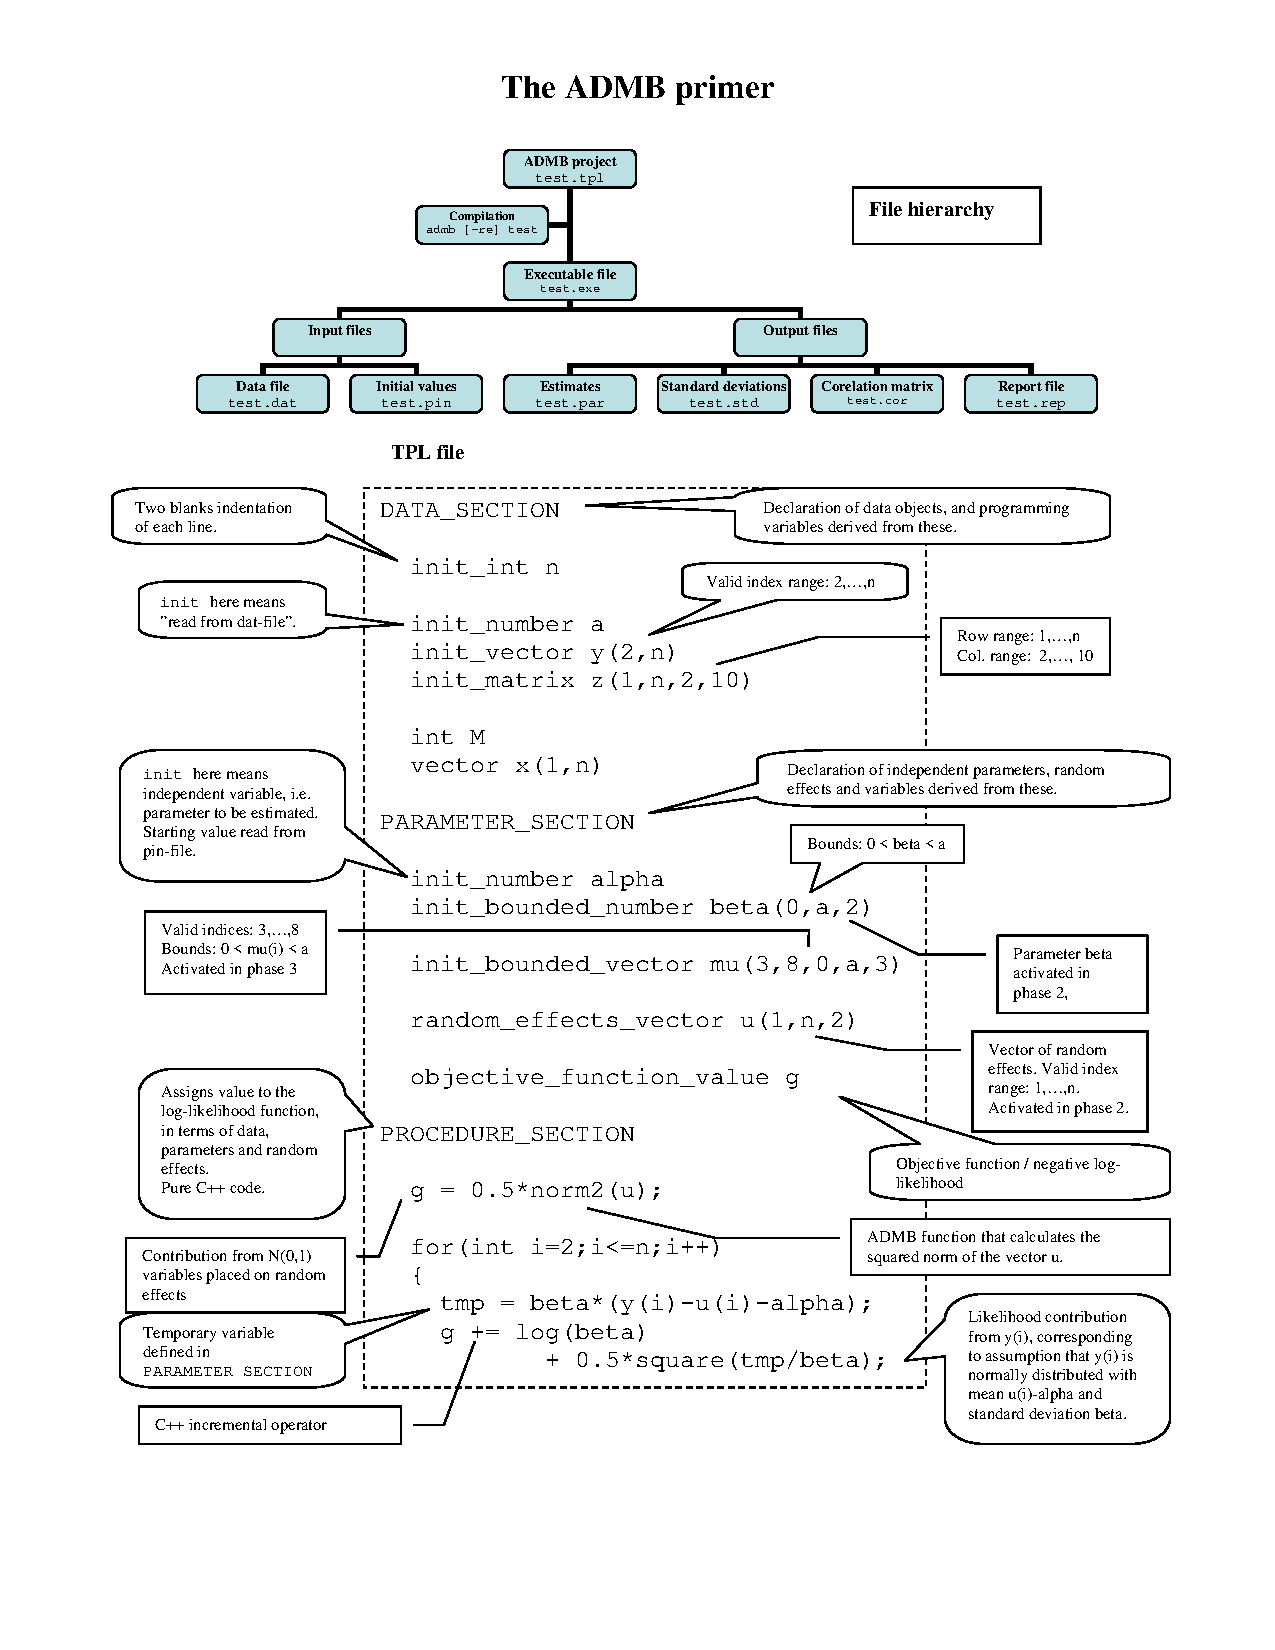
\includegraphics[width=17cm]{ADMBprim.pdf}
\end{figure}

\vskip-4cm
\begin{figure}[H]
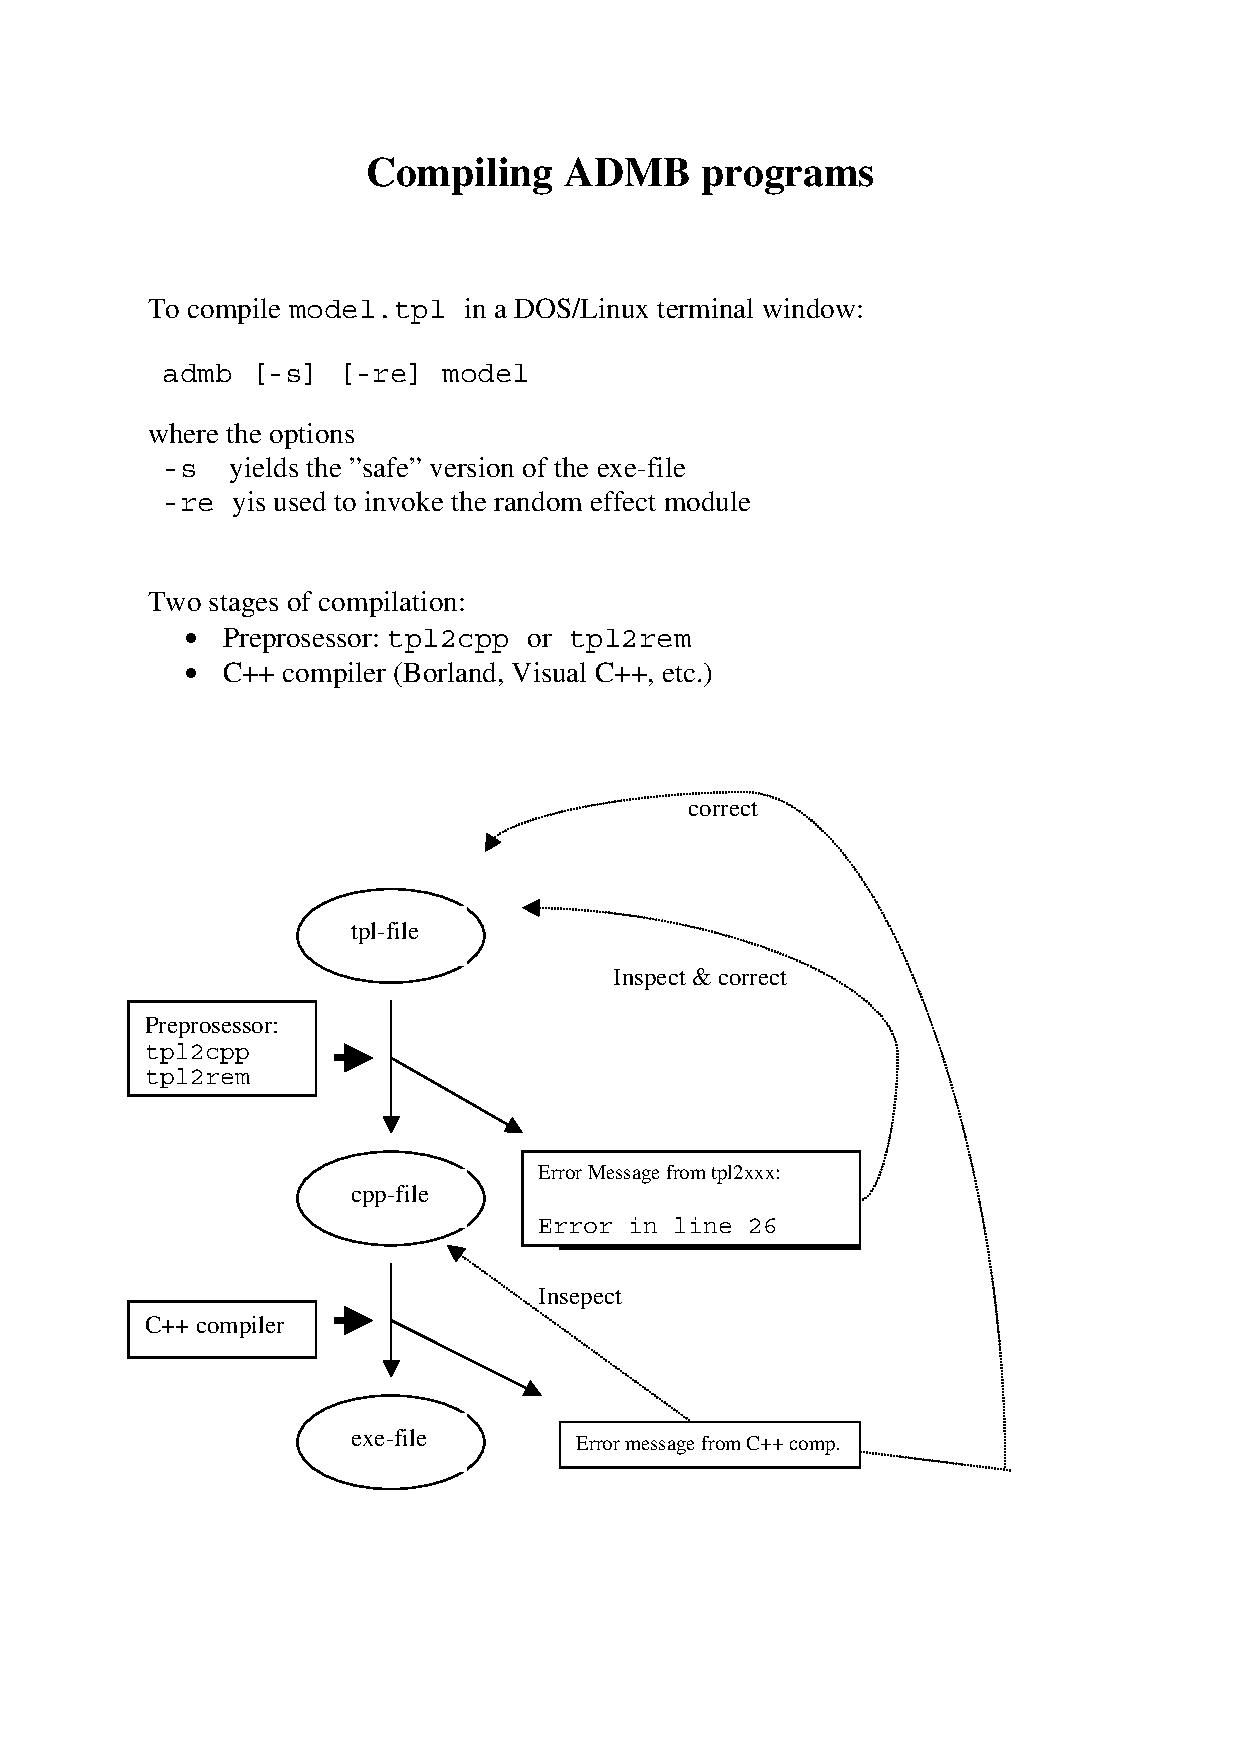
\includegraphics[width=17cm]{compiling.pdf}
\end{figure}

\bibliographystyle{agsm}
\bibliography{skaug}


 \printindex

\end{document}
